\chapter{Lec 16 - Graph Neural Networks}

\section{Introduction}
Traditional ML approaches have been developed assuming data to be encoded into feature vectors; however, many important real-world applications generate data that are naturally represented by more complex structures, such as graphs. Graphs are particularly suited to
represent the relations (arcs) between the components (nodes) constituting an entity. For instance, in social network data, single data “points” (i.e., users) are closely inter-related.\newline\newline
A graph $G = (V, E)$ can be represented using the so called \textbf{adjacency matrix}. A $n \times n$ matrix $A$ such that $A[i,j] = 1$ if $edge(i,j) \in E$, 0 otherwise.\newline\newline
    \textbf{Example:}\newline\newline
    \begin{center}
        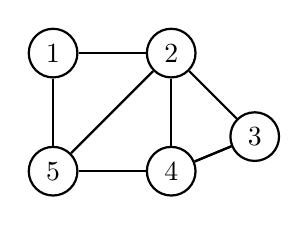
\begin{tikzpicture}[node distance={15mm}, thick, main/.style = {draw, circle}] 
            \node[main] (1) {$1$}; 
            \node[main] (2) [right of=1] {$2$}; 
            \node[main] (3) [below right of=2] {$3$}; 
            \node[main] (4) [below of=2] {$4$}; 
            \node[main] (5) [below of=1] {$5$}; 
            \draw (1) -- (2); 
            \draw (1) -- (5); 
            \draw (2) -- (5);
            \draw (2) -- (4);
            \draw (5) -- (4);
            \draw (3) -- (4); 
            \draw (5) -- (4);
            \draw (4) -- (3);
            \draw (2) -- (3);
        \end{tikzpicture}
    \end{center}
    The Adjacency matrix of the graph above is the following:
    \[\begin{bmatrix}
        0 & 1 & 0 & 0 & 1 \\
        1 & 0 & 1 & 1 & 1 \\
        0 & 1 & 0 & 1 & 0 \\
        0 & 1 & 1 & 0 & 1 \\
        1 & 1 & 0 & 1 & 0
    \end{bmatrix}\]
In undirected graphs this matrix is \textbf{symmetric}, while in directed graphs it is \textbf{asymmetric}. In case of a weighted graph, each cell of the matrix has either the value of the edge weight $w$ or $-$. Each node and edge is represented by a feature vector:
\begin{center}
    \includegraphics[scale=0.5]{images/graphs.png}
\end{center}
The position $(m,n)$, of the adjacency matrix contains the number of walks of length one from node $m$ to node $n$. Position $(m,n)$ of the \textbf{squared} adjacency matrix $A^2$ contains the number of walks of length two from node $m$ to node $n$.\newline\newline
The main problem settings that can arise when dealing with structured data are the following:
\begin{itemize}
    \item Predictions over \textbf{nodes} in a network: In this setting, the dataset is composed of a single (possibly disconnected) large graph. Each example is a node in the graph, and the learning tasks are defined as predictions over the nodes. Given an unseen node $u$, the task is to predict the correct target $y_u$. An example in this setting is the prediction of properties of a social network user based on his or her connections.

    \item Predictions over \textbf{graphs}: In this case, each example is composed of a whole graph, and the learning tasks are predictions of properties of the whole graphs. An example is the prediction of toxicity in humans of chemical compounds represented by their molecular graph.

    \item Link-prediction tasks: the model predicts whether or not there should be an edge between nodes. 
\end{itemize}

\section{Learning on graphs is difficult}
Let $\textbf{X}$ be the matrix in which the feature vectors of each node are stored. We can observe that node indexing in graphs is arbitrary. This means that, differently from images, permuting the node indices results in a permutation of the columns of $\textbf{X}$ and a permutation of both the rows and columns of $A$. However, the underlying graph is unchanged. This property is called Permutation Invariance. More formally, given a permutation matrix $\textbf{P}$, we get a different representation of the same graph:
\[\begin{split}
    \textbf{X}' & = \textbf{XP}\\
    \textbf{A}' & = \textbf{P}^T \textbf{AP}
\end{split}
\]
This property can give the intuition about why learning on graphs is difficult. In fact, determining if two graphs are equal (graphs isomorphism) is a problem for which are not known polynomial-time algorithms. Furthermore, sub-graph isomorphism, which is the problem of determining if a graph is a sub-graph of another graph, is NP-Complete. These problems affect machine learning because a model should be able to predict the same output for isomorphic graphs (which can be represented in different ways). Furthermore, the model we design should capture the similarity between two graphs (sub-graph isomorphism).\newline\newline
In general, the main problems we face when learning on graphs are the following:
\begin{enumerate}
    \item Same graph can be represented in different ways;
    \item How to recognize that a given graph $G_2$ is a sub-graph of $G_1$
    \item How to represent graphs of different sizes (i.e., different number of nodes) into fixed-size vectors without loosing expressiveness ?

    \item How to avoid explosion in the number of parameters with the size of the graphs?
    
\end{enumerate}
Problem 3 is commonly faced by using recursive models that exploit a
causal state space [Sperduti \& Starita., TNN 1997], while Problem 4  is commonly faced by exploiting shared parameters.\newline\newline
Regarding Problems 1 and 2, a sound and meaningful representation for graphs can be achieved by using a neural network with \textbf{convolution operator}, defined on graphs.

\section{Graph Neural Networks - General Idea}
A Graph Neural Network (GNN) receives in input a graph (adj. matrix and node representations. for simplicity) and passes it through a series of $k$ layers. Each layer computes a hidden representation for each node, with the last layer computing the final nodes' embeddings $\textbf{H}_k$. Similarly to CNNs, each node representation includes information about the node and its context within the graph.
\begin{itemize}
    \item For \textbf{node-level tasks}, the output is computed from $\textbf{H}_k$;

    \item For \textbf{graph-level tasks}, the nodes' embeddings are combined (e.g., by averaging), and the resulting vector is mapped via a linear transformation or neural network to a fixed-size vector from which the classification/regression task is performed.

    \item For \textbf{link-prediction tasks}, the embeddings of the two endpoint nodes must be mapped to a single number representing the probability that the edge is present (e.g. dot product of the nodes' embeddings and pass the result through a sigmoid function to create a probability).
 
\end{itemize}
\begin{center}
    \includegraphics[]{images/gnn.png}
\end{center}

\section{Graph Convolution}
The general idea of graph convolution starts from a parallel between graphs and images. GNNs implement convolution in a similar way how CNNs do, that is, learning the features by inspecting neighboring nodes. GNNs generalize the definition of convolution for non-regular structured data.

\subsection{NN4G by Micheli}
\textbf{NN4G} is an architecture based on a graph convolution that is defined as:
\begin{center}
    \includegraphics[scale=0.6]{images/nn4g.png}
\end{center}
where: 
\begin{itemize}
    \item $\sigma$ is a nonlinear activation function applied element-wise.
    \item $N(v)$ represent the neighborhood of node $v$.
    \item $\textbf{W}^i$ is a weights' matrix;
    \item $\textbf{x}_u$ is the feature vector of node $u$.
\end{itemize}
Actually, this is a simplified notation, since the original one uses skip connections (see GNN book chapter).
\begin{center}
    \includegraphics[]{images/nn4g-2.png}
\end{center}
Note that:
\begin{itemize}
    \item The first layer ($i = 1$), which has no previous layers, computes the nodes' representations only on the basis of each vertex feature vector.

    \item Each convolution performed on the $i$-th hidden units, with $i > 1$, takes as input the neighbors' representations of the previous layer. Basically, it merges the representations of each node with those of its neighbors:

    \item $X_1(g), X_2(g), X_3(g)$ are scalar values computed by aggregating the representations $\textbf{x}_i(g)$ for each unit $i$.
    In particular they are defined as:
    \[X_i(g) = \frac{1}{k}\sum_{v \in Vert(g)}x_i(v)\]
    if $k = 1$, this corresponds to a sum. Basically, we compute a representation per-graph per-layer. Then, this 3 representations are parametrized by the weights $w_1, w_2, w_3$ and used to compute the output for the whole graph (graph-level task).
\end{itemize}
The convolutional operation presented above can be defined in a compact way using matrix multiplications:
\begin{center}
    \includegraphics[scale=0.6]{images/matrix-gcn.png}
\end{center}
where $\textbf{A}$ is the adjacency matrix. Exploiting matrix multiplications makes the computation really fast. Furthermore, note that, as for images, the receptive field of the layers increases as we stack more layers.\newline\newline
Note also that, since with the convolution operator we are merging neighboring nodes' representations, isomorphic graphs in which the order of the nodes is changed will have the same nodes' representations.

\subsection{Graph Fourier Transform}
The operation described above is graph convolution, but how it is derived? Defining the formal convolution operator on graph is difficult.\newline\newline
Let $x: V \rightarrow \mathbb{R}$ be a signal on the nodes $V$ of the graph $G$, i.e., a function that associates a real value with each node of $V$. We can represent every signal as a vector $\textbf{x} \in \mathbb{R}^n$, which from now on we will refer to as signal. In order to set up a convolutional network on $G$, we need the notion of convolution between a signal $\textbf{x}$ and a filter signal $\textbf{f}$.\newline\newline
The key idea is to use a Fourier transform. In the frequency domain, thanks to the \textbf{Convolution Theorem}, the (undefined) convolution of two signals becomes the (well-defined) component-wise product of their transforms. So, if we knew how to compute the Fourier transform of a function defined on a graph, we could define the convolution operator.\newline\newline
The Convolution Theorem states that convolution in one domain (time, space) corresponds to pointwise multiplication in frequency domain.\newline\newline
The \textbf{graph Fourier transform} is defined starting from the (normalized) Laplacian matrix of the graph, which is defined as:
\[L = I_n - D^{-\frac{1}{2}} A D^{-\frac{1}{2}}\]
where:
\begin{itemize}
    \item $I_n$ is the identity matrix;
    \item $A$ is the adjacency matrix;
    \item $D$ is the degree matrix, that is, the \textbf{diagonal} matrix containing the number of edges attached to each vertex;
\end{itemize}
Then, we can compute the eigendecomposition of $L$ (which is always possible):
\[L = U \Lambda U^T\]
where $\Lambda = diag([\lambda_0, ..., \lambda_{n-1}])$ and $U$ is the Fourier basis of the graph.\newline\newline
Finally, Given a spatial signal $\textbf{x}$:
\begin{itemize}
    \item $\hat{\textbf{x}} = U^T\textbf{x}$ is its graph Fourier Transform

    \item $\textbf{x} = U \hat{\textbf{x}}$ is the inverse Fourier transform
\end{itemize}
Therefore, convolution between a parametric filter and a signal can be defined as:
\[y = \textbf{f}_\theta *_G \textbf{x} = U\left( (U^T\textbf{f}_\theta) \odot (U^T \textbf{x})\right)\]
It can be proved that this operator corresponds to the one used for NN4G presented previously (see slides for more details).

\section{Aggregation Layer for graph classification}
With Graph Convolution we have a representation for each graph node. How can we map node representations to a graph-level representation? There are some simple solutions, like the sum or the average of nodes' representations as we saw previously, or we can rely on more complex alternatives: Universal readout.


\section{Graph Recurrent Neural Networks}
Scarselli et al. proposed a network architecture where, instead of stacking multiple layers, a single recurrent layer is adopted:
\[\textbf{h}_v^{t+1} = \sum_{u \in N(v)}f(\textbf{h}_u^t, \textbf{x}_v, \textbf{x}_u)\]
where $f$ is a function (e.g. neural network) with shared parameters across all the nodes and all the time steps. The recurrent system is defined as a contraction mapping, and thus it is guaranteed to converge to a fixed point $\textbf{h*}$.

\subsection{Gated Graph Neural Networks}
The idea is to remove the constraint for the recurrent system to be a contraction mapping, and implement this idea by adopting recurrent
neural networks to define the recurrence. Specifically, the gated recurrent unit (GRU) is adopted. The recurrent convolution operator is defined as follows:
\begin{center}
    \includegraphics[scale=0.8]{images/gated-gnn.png}
\end{center}
where $\textbf{A}_v$ is row $v$ of the adjacency matrix $\textbf{A}$.

